\chapter{Modèle et entraînement}\label{chap:modele}

Ce chapitre décrit l’architecture complète du classifieur, la procédure d’entraînement en deux phases et les choix d’hyperparamètres. Le code correspondant est donné en annexe~\ref{app:code}.

\section{Architecture du modèle}

Le modèle enchaîne cinq blocs, de l’image brute aux probabilités (figure~\ref{fig:modele})~:

\begin{enumerate}
  \item l’\textbf{entrée}~: une image $224\times224\times3$ dont les pixels sont des flottants entre 0 et 255~;
  \item le bloc d’\textbf{augmentation} (retournements, rotation, zoom, luminosité, contraste), actif seulement à l’entraînement~;
  \item le \textbf{prétraitement} MobileNetV2~: division par 127,5 puis soustraction de 1, pour obtenir des valeurs dans $[-1,1]$ ;
  \item la \textbf{base MobileNetV2} pré-entraînée sur ImageNet, sans sa tête, qui produit une carte de caractéristiques $7\times7\times1280$ ;
  \item la \textbf{tête de classification}~: pooling moyen global ($1280$ valeurs), dropout de taux $0{,}3$, couche dense à 11 sorties avec softmax.
\end{enumerate}

\begin{figure}[H]
\centering
\begin{tikzpicture}[node distance=3mm]
  \node[blkw,minimum width=19mm,minimum height=17mm] (a) {\textbf{Image}\\[-1pt]\scriptsize $224{\times}224{\times}3$\\0--255};
  \node[blko,minimum width=21mm,minimum height=17mm,right=of a] (b) {\textbf{Augmen-}\\\textbf{tation}\\[-1pt]{\scriptsize (train seul.)}};
  \node[blk,minimum width=19mm,minimum height=17mm,right=of b] (c) {\textbf{Prétrait.}\\[-1pt]{\scriptsize $[-1,1]$}};
  \node[blk,minimum width=24mm,minimum height=17mm,right=of c,fill=navy!14] (d) {\textbf{MobileNetV2}\\[-1pt]\scriptsize $7{\times}7{\times}1280$\\2\,257\,984 param.};
  \node[blk,minimum width=21mm,minimum height=17mm,right=of d] (e) {\textbf{GAP +}\\\textbf{Dropout 0,3}\\[-1pt]{\scriptsize 1280}};
  \node[blkg,minimum width=21mm,minimum height=17mm,right=of e] (f) {\textbf{Dense 11}\\[-1pt]\scriptsize softmax\\14\,091 param.};
  \foreach \x/\y in {a/b,b/c,c/d,d/e,e/f} \draw[arr] (\x) -- (\y);
\end{tikzpicture}
\caption{Architecture complète du classifieur de maturité.}\label{fig:modele}
\end{figure}

\paragraph{Nombre de paramètres.} La tête contient $1280\times 11 + 11 = 14\,091$ paramètres (poids plus biais). Ajoutée aux $2\,257\,984$ paramètres de la base, elle porte le total à \textbf{2\,272\,075} paramètres. Plus de 99\,\% du modèle provient donc de la base pré-entraînée.

\begin{table}[H]
\centering
\caption{Répartition des paramètres.}\label{tab:params}
\small
\begin{tabular}{@{}lrr@{}}
\toprule
\textbf{Partie} & \textbf{Paramètres} & \textbf{Part} \\
\midrule
Base MobileNetV2 (sans tête) & 2\,257\,984 & 99,4\,\% \\
Tête (dense $1280\to 11$) & 14\,091 & 0,6\,\% \\
\midrule
\textbf{Total} & \textbf{2\,272\,075} & 100\,\% \\
\bottomrule
\end{tabular}
\end{table}

\section{Fonction de perte et métrique}

La perte est l’\textbf{entropie croisée catégorielle} (chapitre~\ref{chap:dl}), calculée sur les étiquettes entières (\code{sparse\_categorical\_crossentropy}) et pondérée par les poids de classes de la section~\ref{sec:poids}. La métrique suivie pendant l’entraînement est l’exactitude (proportion d’images correctement classées).

\section{Phase 1~: entraînement de la tête}

Dans la première phase, la base MobileNetV2 est \textbf{gelée}~: ses poids ne changent pas. Seule la tête de 14\,091 paramètres est entraînée. Les caractéristiques extraites par la base sont déjà très riches~; la tête apprend simplement à les combiner pour reconnaître nos 11 classes.

\begin{itemize}
  \item optimiseur \textbf{Adam}, taux d’apprentissage $10^{-3}$ ;
  \item au plus \textbf{25 époques}, lots de 32 images~;
  \item \textbf{EarlyStopping} sur la perte de validation (patience 6), avec restauration des meilleurs poids~;
  \item \textbf{ReduceLROnPlateau}~: le taux est divisé par deux si la perte de validation stagne pendant 3 époques.
\end{itemize}

Le gel de la base est cohérent avec la logique du transfert~: avec un taux élevé, des gradients issus d’une tête initialisée au hasard abîmeraient les poids pré-entraînés. La phase 1 se termine après une douzaine d’époques, avec une exactitude de validation d’environ 91\,\%.

\section{Phase 2~: fine-tuning}\label{sec:finetune}

Dans la deuxième phase, nous \textbf{dégelons les 40 dernières couches} de la base et continuons l’entraînement avec un taux d’apprentissage beaucoup plus faible, afin d’adapter finement les caractéristiques de haut niveau aux fruits sans détruire ce qui a été appris sur ImageNet.

\begin{itemize}
  \item optimiseur Adam, taux d’apprentissage \textbf{$10^{-5}$} (cent fois plus faible)~;
  \item au plus \textbf{40 époques}~;
  \item EarlyStopping sur la perte de validation (patience 10) et ReduceLROnPlateau (facteur 0,5, patience 4, taux minimal $10^{-7}$)~;
  \item \textbf{couches de normalisation par lots gelées}~: parmi les couches dégelées, les couches BatchNormalization restent figées.
\end{itemize}

\begin{keybox}{Pourquoi geler la BatchNormalization~?}
Ces couches maintiennent des moyennes et variances mobiles calculées sur ImageNet. En fine-tuning sur un petit jeu de données et de petits lots, mettre à jour ces statistiques les rend instables et dégrade la précision. Les laisser figées est la pratique recommandée par la documentation de Keras, et cette précaution, associée à la correction des callbacks décrite plus bas, a fait passer notre exactitude de test de 90,0\,\% à 93,1\,\% (chapitre~\ref{chap:resultats}, expériences 1 et 2).
\end{keybox}

\section{Courbes d’apprentissage}

La figure~\ref{fig:courbes} montre l’évolution de l’exactitude et de la perte au fil des époques. L’exactitude de validation monte rapidement pendant la phase 1 (environ 91\,\%), puis progresse plus lentement pendant le fine-tuning pour se stabiliser autour de 92\,\%. L’exactitude d’entraînement atteint environ 97\,\%.

\begin{figure}[H]
\centering
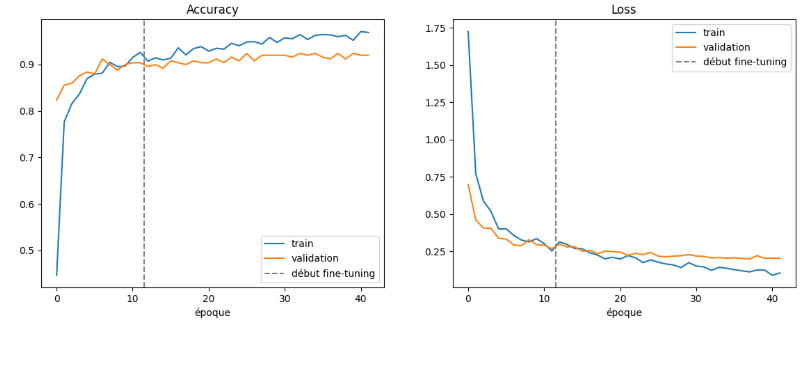
\includegraphics[width=0.96\textwidth]{figures/courbes.png}
\caption{Courbes d’apprentissage~: exactitude et perte, entraînement et validation, phases 1 et 2.}\label{fig:courbes}
\end{figure}

\paragraph{Lecture.} L’écart d’environ cinq points entre l’entraînement (97\,\%) et la validation (92\,\%) indique un \textbf{surapprentissage modéré} : le modèle s’adapte un peu mieux aux images qu’il a vues qu’aux nouvelles. Il n’est pas catastrophique, car la perte de validation ne remonte pas, et il est atténué par l’arrêt anticipé et le dropout. Avec seulement 1\,118 images d’entraînement, il est difficile de le réduire davantage sans nouvelles données.

\section{Hyperparamètres retenus}

\begin{table}[H]
\centering
\caption{Récapitulatif de la configuration de l’entraînement.}\label{tab:hyper}
\small
\begin{tabular}{@{}p{5.2cm}p{4.5cm}p{3.8cm}@{}}
\toprule
\textbf{Paramètre} & \textbf{Phase 1} & \textbf{Phase 2} \\
\midrule
Couches entraînées & Tête uniquement & 40 dernières couches de la base + tête (BatchNorm gelées) \\
Optimiseur & Adam & Adam \\
Taux d’apprentissage & $10^{-3}$ & $10^{-5}$ \\
Époques maximales & 25 & 40 \\
Taille de lot & 32 & 32 \\
EarlyStopping (val\_loss) & patience 6 & patience 10 \\
ReduceLROnPlateau & ×0,5, patience 3 & ×0,5, patience 4 \\
Dropout & 0,3 & 0,3 \\
Poids de classes & \multicolumn{2}{c}{«~balanced~» (0,56 à 3,08)} \\
Entrée & \multicolumn{2}{c}{$224\times224\times3$, pixels 0--255} \\
\bottomrule
\end{tabular}
\end{table}

\section{Un piège rencontré~: la réutilisation des callbacks}

Notre première tentative a donné 90,0\,\%. Deux corrections ont ensuite été apportées. D’abord, les mêmes objets \code{callbacks} avaient été réutilisés dans les deux phases ; or EarlyStopping conserve en mémoire la meilleure valeur observée et son compteur de patience. En phase 2, il comparait la perte de validation à la meilleure valeur de la phase 1 et pouvait donc stopper l’entraînement trop tôt. Nous créons maintenant de nouveaux objets pour chaque phase. Ensuite, nous avons gelé les couches BatchNormalization pendant le fine-tuning (encadré précédent). Ces deux corrections ont donné le modèle retenu à 93,1\,\%.

\section{Environnement de calcul}

L’entraînement a été exécuté sur Kaggle avec deux GPU NVIDIA T4. Une époque dure environ 3 à 4 secondes (environ 35 lots de 32 images), si bien que la procédure complète tient en quelques minutes. Cette rapidité permet d’explorer plusieurs variantes, comme nous l’avons fait au chapitre suivant.
